\chapter{Methods}

An overview of the approach used in this study is provided in Figure \ref{fig:methodsoverview}.
The main computational discovery pipeline uses data curated from public datasets to search for conserved structured RNA elements encoded near a conserved protein domain anchor.
Conversely, the positive control pipeline searches for conserved protein domains starting from a known RNA element anchor, acting to validate both the discovery pipeline and the premise of this project.

In addition to the main discovery and positive control pipelines, iterative expansion and covariance model clustering approaches are described as downstream analyses for identified candidates.

\begin{figure}[H]
    \centering
    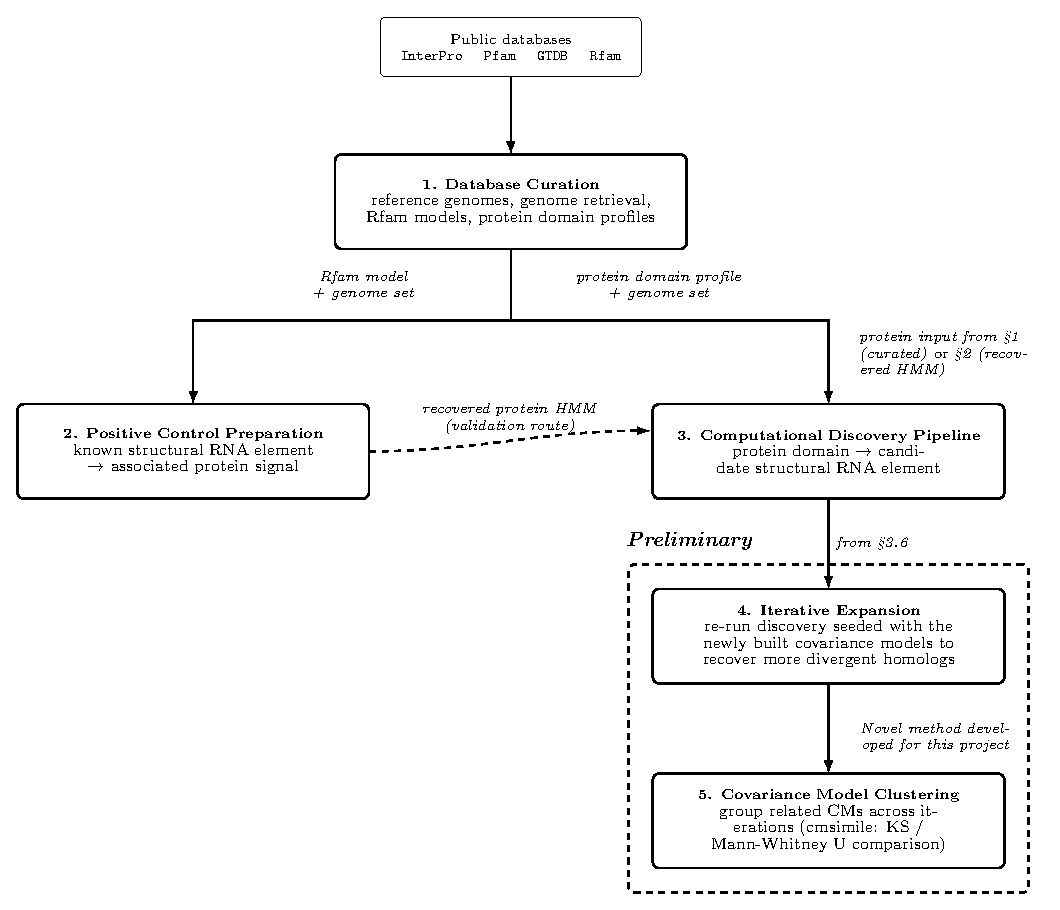
\includegraphics[width=0.95\textwidth]{figures/methods/overview.pdf}
    \caption[Overview of methods]{\textbf{Overview of methods}
    Simplified overview of the approach taken for \ac{RNP} candidate discovery. Numbered steps refer to the following subsections. }
    \label{fig:methodsoverview}
\end{figure}

The discovery and positive control pipelines are written in Python 3.14.6 using Snakemake v.9.23.1, and are configurable and automated \citep{Molder2025}.
Iterative expansion and covariance model clustering were developed in Go v.1.27.1 and are available as standalone tools.
All code, software environment definitions and data used in this study are available in the supplementary materials (Appendix \ref{sec:code-and-data-availability}).

\section{Database curation}

% abstract steps from discovery and positive control pipeline, and describe the databases used and versions.

% \begin{figure}[H]
%     \centering
%     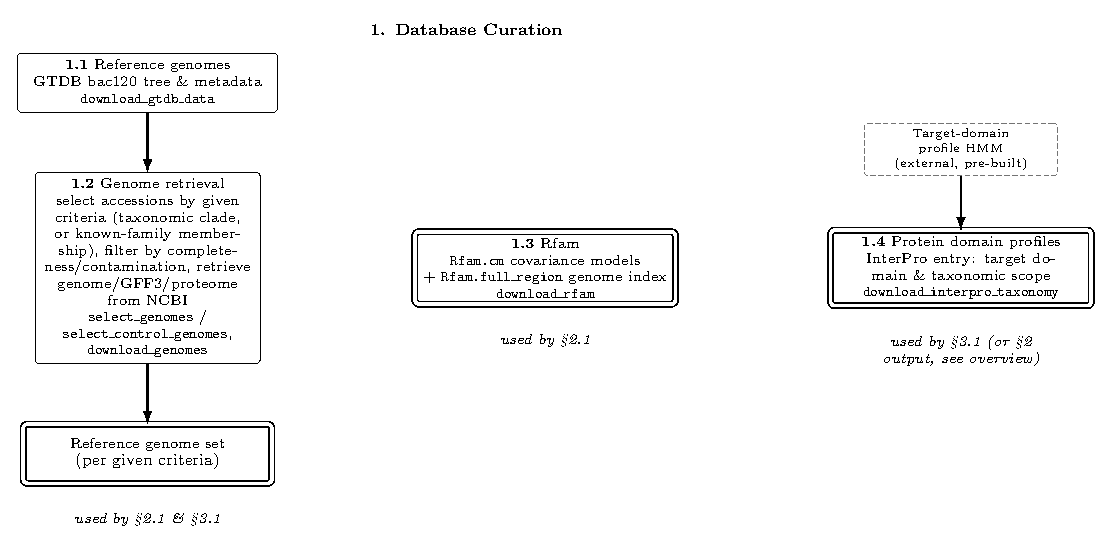
\includegraphics[width=0.95\textwidth]{figures/methods/section1_database_curation.pdf}
%     \caption[Database curation]{\textbf{Database curation}
%     An overview of the databases used and filtering and curation steps taken. 
%     Numbered steps refer to the subsections below. 
%     In bold are custom script and assets retrieved from online public databases.}
%     \label{fig:databasecuration}
% \end{figure}



\subsection{Reference genomes}
\label{subsec:reference-genomes}

For all analyses, the \ac{GTDB} release 232 \citep{Parks2022} was used to select a diverse set of bacterial genomes for analysis. 
The GTDB provides a standardised taxonomy, ensuring that the selected genomes are representative of the bacterial domain. 
Python package ete3 v.3.1.3 \citep{huertacepas2016} was used for phylogenetic analysis and filtering using the \ac{GTDB} phylogenetic tree.
Further filtering was performed to select high-quality, complete genomes (completeness $>$ 99.9\%, contamination $<$ 1\%), ensuring the selected reference genomes are suitable for downstream analysis.
Completeness and contamination metrics were provided by CheckM2 \citep{Chklovski2023}, available in the \ac{GTDB} release.

\subsubsection{Genome retrieval}
\label{sec:genomes}

Only genomes with genomic sequence, protein sequence and annotation files available were retrieved from the \ac{NCBI} GenBank database release 265.0 \citep{OLeary2024}.

Full lists of genomes used in this study for particular experiments are available in the supplementary materials (Appendix \ref{sec:code-and-data-availability}).

\subsection{Covariance models}
\label{subsec:covariance-models}

RNA family covariance models were retrieved from the Rfam database (version 15.0) \citep{Ontiveros-Palacios2025}.
These were used in positive control experiments to validate the pipeline and to identify known RNA families among the candidates identified.

Additionally, covariance models and clan information available from the Rfam database (version 15.0) \citep{Ontiveros-Palacios2025} were used to validate the clustering method developed in this study.
Seed sequences (curated members of each family, used to build the alignments from which the family models are built) were also retrieved.

\subsection{Protein domain profiles}
\label{subsec:protein-hmm-retrieval}

InterPro (version 35.0) entries guided the choice of protein domain model and relevant genome search space \citep{Blum2025}.
Protein domain \ac{HMM} profiles were retrieved from the Pfam v.35.0 database \citep{Paysan-Fafosse2025}.
These were used in the discovery pipeline to search for protein homology to anchor the search for conserved structured RNA elements.

% -------- rna -> protein ------------

\section{Positive control preparation}
\label{sec:poscontrol-pipeline}


\begin{figure}[htbp]
    \centering
    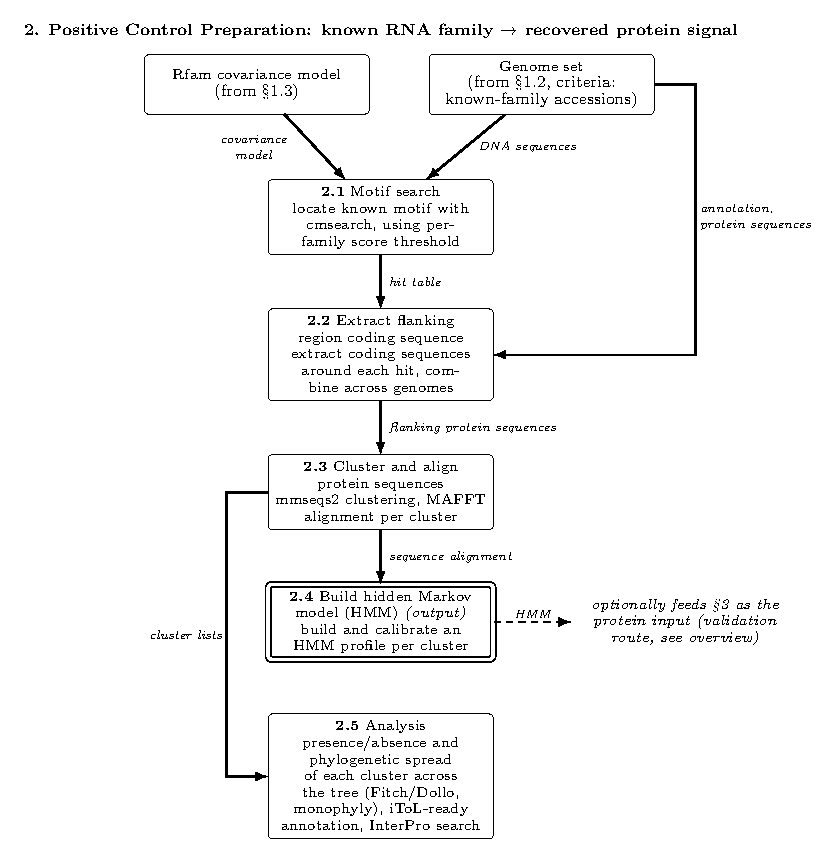
\includegraphics[width=0.95\textwidth]{figures/methods/section2_positive_control.pdf}
    \caption[Positive control preparation] {\textbf{Positive control preparation (known RNA family $\rightarrow$ recovered protein signal).}
    Starting from Rfam covariance models (\S\ref{subsec:covariance-models}) and genomes containing known family members (\S\ref{sec:genomes}), the pipeline locates each known element with cmsearch, extracts
    the flanking coding sequences, and clusters and aligns the encoded proteins. 
    Coding sequences within 1000\,nt of each hit were extracted. 
    Proteins were clustered with MMseqs2 (sensitivity 7.5, minimum sequence identity 0.25, coverage $\geq 0.2$), and clusters with fewer than 5 members were discarded.
    Italic labels show the data passed between steps. A hidden Markov model is built and calibrated for each cluster (double border, output) and can optionally feed the discovery pipeline as the protein input. 
    Clusters are also analysed for presence/absence and phylogenetic spread across the tree, and searched against InterPro.
    Hits were called using the Rfam per-family score thresholds and covariance models.}
    \label{fig:poscontrol}
\end{figure}

Pipeline inputs are Rfam covariance models and annotated seed sequences, as described in Section~\ref{subsec:covariance-models}.
A custom script accessing Entrez via the Python Biopython v.1.87 library searches for genomes containing these sequences \citep{OLeary2024}.
A genome set is then constructed from \ac{GTDB} reference genomes and downloaded from GenBank (Section~\ref{subsec:reference-genomes}).
All inputs from runs of this pipeline used in this study are available in Table \ref{tab:positive_controls_input}.

\subsection{RNA structure search}

Members of the Rfam family were searched using the Rfam published search parameters, to revalidate hits and confirm coordinate system in reference genomes (Infernal v.1.1.5 \emph{cmsearch}).
The output of this step is a list of genomic coordinates for each hit, which is used to extract the flanking coding sequences.

\subsection{Extract flanking coding sequences}

Coding sequences surrounding the RNA element locus are extracted from the genome, within a 1000 nucleotide region.
This was done to identify protein domains that are encoded in close proximity to the RNA element, which may indicate a functional relationship between the two.
The approach is illustrated in Figure \ref{fig:flankingcds}.

\begin{figure}[H]
    \centering
    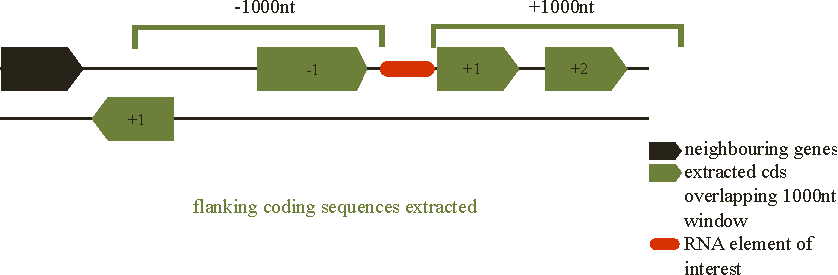
\includegraphics[width=0.8\textwidth]{figures/methods/flanking_cds_fig.pdf}
    \caption[Flanking coding sequence extraction]{\textbf{Flanking coding sequence extraction.}
    Annotated coding sequences surrounding the RNA element of interest are extracted from genomes within a 1000 nucleotide region.
    Shown in red is the RNA element of interest identified by cmsearch, in black is a coding sequence outside the 1000 nucleotide extraction region.
    Indicated in green are the flanking coding sequences extracted for further analysis, labelled by upstream (+) or downstream (-) of the RNA element as well as the order (1 or 2 upstream or downstream). 
    Strandedness of the surrounding coding sequences is also recorded (same or different to the cmsearch hit).}
    \label{fig:flankingcds}
\end{figure}

Reference genome annotation files were used to identify the coding sequences flanking the RNA element of interest, using coordinates from the RNA structure search output by a custom script.
Protein sequences of these identified coding sequences were then extracted from the genome and used for downstream clustering and alignment.

\subsection{Clustering and aligning protein sequences}

\subsubsection{Clustering}

Protein homology was assessed by clustering the extracted protein sequences.
Protein sequences were clustered using MMseqs2 v.14.7.0 \citep{Steinegger2017}.
The clustering was performed with a sensitivity of 7.5, a minimum sequence identity of 0.25, and a minimum coverage of 0.2.
Clusters with fewer than 5 members were discarded to ensure that only clusters with sufficient representation were retained for further analysis.

\subsubsection{Sequence alignment}

A \ac{MSA} was built using from the trimmed cluster sequences (MAFFT v.7.525) \citep{Katoh2013}.
This identifies conserved sequence features and provides a basis for secondary structure prediction and covariance model building.
Alignments also describe how sequences are related to each other, which is important for downstream analyses such as covariance model building and iterative expansion.


\subsection{Build \ac{HMM}}
\label{sec:positive_control_hmm}

Probabalistic models, \ac{HMM}s, were built based on the \ac{MSA} of each alignment.
This was done to capture the sequence diversity of each cluster, and to allow for sensitive searches for homologous sequences in the discovery pipeline.
HMMER v.3.4 \emph{hmmbuild} and \emph{hmmcalibrate} were used to build and calibrate the \ac{HMM}s.

\subsection{Analysis}

The pipeline reports the results of the computational analysis, the prevelence of cluster members across the reference genomes.
The position of the protein domain relative to the RNA element is also reported, as well as the number of clusters identified and their sizes.

\subsubsection{Taxonomic spread analyses with \ac{iTOL}}

Monophylicity or polyphylicity of clusters was assessed by mapping the presence or absence of cluster members to the \ac{GTDB} phylogenetic tree.

An annotation file was generated for each cluster, indicating the presence or absence of a cluster member in each genome.
This was visualised on the \ac{iTOL} v.7 online tool \citep{Letunic2024} to assess the taxonomic spread of each cluster, and identify bacterial clades where the cluster is more abundant for positive control inputs of the discovery pipeline.

\subsubsection{Identification with InterPro}

Cluster sequences were submitted to the online InterProScan v.6 tool; the results indicated the protein hits and what the protein signal represents \citep{Blum2026}.
Pfam v.35.0 entries were reported for the highest prevalence cluster, and the InterPro entry was used to identify the protein domain represented by the cluster.

% -------- protein -> rna ------------

\section{Computational discovery pipeline}
\label{sec:computational-discovery-pipeline}

\begin{figure}[htbp]
    \centering
    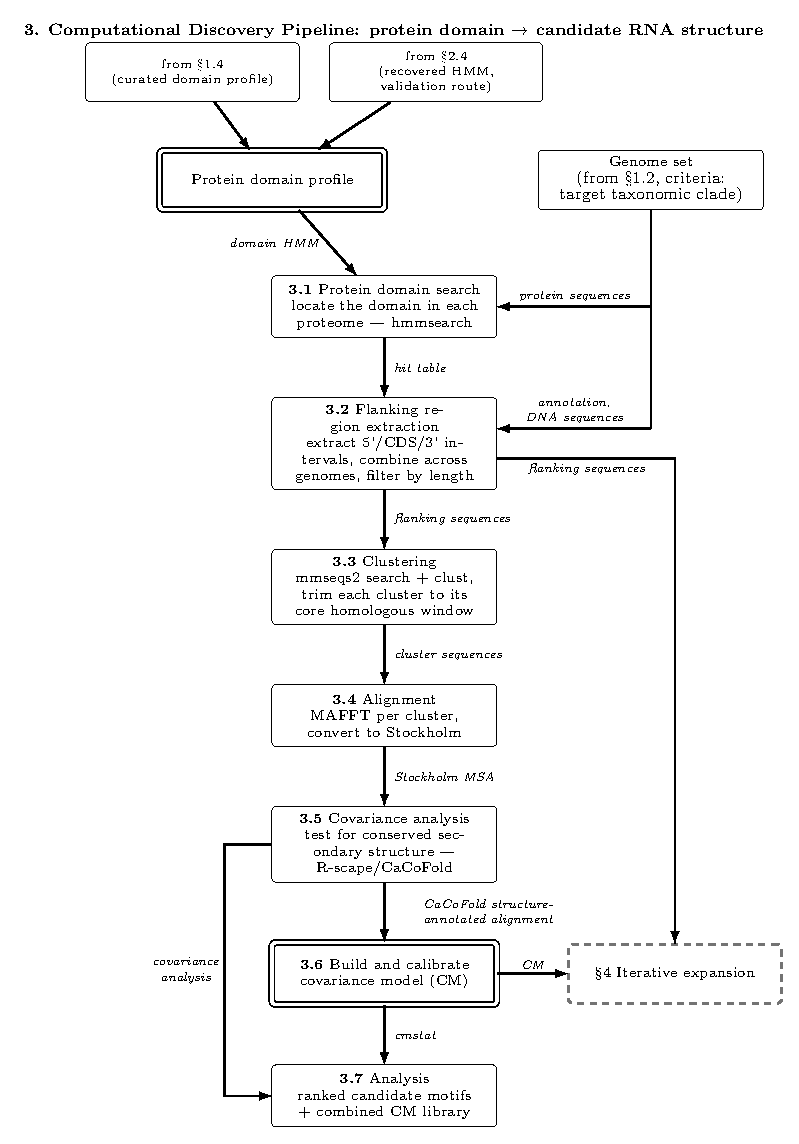
\includegraphics[width=0.95\textwidth, height=0.72\textheight, keepaspectratio]{figures/methods/section3_discovery_pipeline.pdf}
    \caption[Computational discovery pipeline]{%
    \textbf{Computational discovery pipeline (protein domain $\rightarrow$ candidate structured RNA).}
    A protein domain profile, either curated (\S\ref{subsec:protein-hmm-retrieval}) or recovered from the
    positive control (\S\ref{sec:positive_control_hmm}), is searched against the proteomes of the
    target clade (\S\ref{subsec:reference-genomes}). Flanking regions of each hit are extracted, clustered,
    aligned and tested for conserved secondary structure, and covariance models are built from
    the structure-annotated alignments (double border, output). Candidate structured RNAs are
    ranked in the final report, and the covariance models and flanking sequences pass to
    iterative expansion (\S\ref{sec:iterative}). Italic labels show the data passed between
    steps. Filtering thresholds are given in Table~\ref{tab:thresholds}.}
    \label{fig:discovery}
\end{figure}


Inputs of the pipeline are a protein domain \ac{HMM} which serves as an anchor for the search, sourced as described in Section~\ref{subsec:protein-hmm-retrieval}, and a selection of reference genomes as a search space (Section~\ref{subsec:reference-genomes}).
For validation the protein domain \ac{HMM} is one recovered from the positive control pipeline (Section~\ref{sec:poscontrol-pipeline}).
All inputs from runs of this pipeline used in this study are available in Table \ref{tab:discovery_inputs}.

\subsection{Protein domain search}

Protein homology was searched using a probabilistic model (\ac{HMM}) against the genome sequence set (Section~\ref{subsec:reference-genomes}) (\emph{nhmmer} hmmer v3.4).
To narrow the search for structured RNAs, the search was focused to regions flanking the identified protein domains.

\subsection{Flanking region extraction}
\label{sec:flanking}

% describe approach, and filtering done
The flanking regions are extracted from the reference genomes' genomic sequence based on the coordinates of the protein domain hits and the genomic annotations.
The extracted sequences are then filtered for length and quality to ensure that only high-quality sequences are used in subsequent steps.
Figure~\ref{fig:flankingregion} illustrates the flanking region extraction process, where the anchor coding sequence is identified by \emph{nhmmer}, and the annotated up and downstream coding sequences of the same strand are used to define the flanking regions.

\begin{figure}[H]
    \centering
    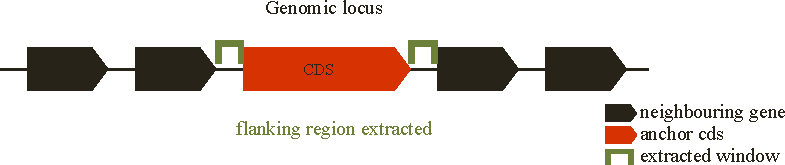
\includegraphics[width=0.8\textwidth]{figures/methods/extracted_flanks.pdf}
    \caption[Flanking region extraction]{\textbf{Flanking region extraction.}
    Non-coding flanking DNA sequence is extracted from genomes based on hmmer hits in protein sequence and published genome annotations.
    Shown in red is the anchor coding sequence identified by nhmmer, in black are annotated up and downstream coding sequences of the same strand.
    Indicated in green are the flanking regions extracted for further analysis. }
    \label{fig:flankingregion}
\end{figure}

Length filtering included only sequences $\geq 20$ nucleotides to allow for meaningful homology searches in subsequent clustering steps.

\subsection{Sequence clustering}

\subsubsection{MMseqs2 clustering}
\label{subsec:clustering}

Flanking sequences were clustered with a pairwise search based on sequence similarity with MMseqs2 v.16.747c6 \emph{search} \citep{Kallenborn2025}.
This was done to group sequences that are likely to be homologous, and to reduce the number of sequences for downstream analyses.

\subsubsection{Sequence trimming}

Clustered sequences are then trimmed to the local-alignment window it shares (directly or transitively) with an anchor sequence from the same cluster, using coordinates from a single all-vs-all search pass (MMseqs2 v.16.747c6).
Window lengths were filtered to include those of length $\geq 15$ and $\leq 1000$ nucleotides.
A padding of 15 nucleotides was kept on either side of this window.
These trimming and filtering steps were implemented to remove spurious flanking sequence and to focus on the conserved region of the cluster.

\subsection{Sequence alignment}
\label{subsec:rna-alignment}

A \ac{MSA} was built using from the trimmed cluster sequences (MAFFT v.7.525) \citep{Katoh2013}.
This identifies conserved sequence features and provides a basis for secondary structure prediction and covariance model building.
Alignments also describe how sequences are related to each other, which is important for downstream analyses such as covariance model building and iterative expansion.

\subsection{Covariance analysis}
\label{subsec:covariance-analysis}

The CaCoFold algorithm of R-scape v.2.0.4 was used to predict conserved secondary structure and covarying base pairs in the \ac{MSA} \citep{Rivas2017}.
This approach tests for covariation in the alignment, and predicts a consensus structure based on the covarying base pairs.
It provides a structure-annotated \ac{MSA} in Stockholm format, which can be used to build a covariance model.
Additionally, it provides a statistical test for covariation, giving an $E$-value for each predicted covarying base pair, statistical power for the covariation test, and an F-value for the overall alignment (the harmonic mean of sensitivity (SEN) and positive predictive value (PPV)).
Secondary structure diagrams were generated with R2R v.1.0.6 \citep{Weinberg2011}.

This covariance analysis step is the key step in the pipeline to identify any structured RNA elements.
$E$-values for covarying base pairs are used to filter out spurious predictions, and the overall F-value is used to assess the quality of the alignment.

\subsection{Covariance model construction and calibration}
\label{sec:build_cm}

Filtering was done on the CaCoFold structurally annotated alignments to include only those with at least one covarying pair where $E \le 0.05$.
The Infernal v.1.1.5 \emph{cmbuild} tool was used to generate probabilistic models from identified CaCoFold generated structural alignments, default parameters were used.
Infernal v.1.1.5 \emph{cmcalibrate} assigns $E$-values to built models by fitting exponential tails to the hits of random sequences, this is required for statistical significance in searches using these models \citep{Nawrocki2013}.
\acp{CM}s with calibration runtimes $< 3$ hours and requiring $< 8$ \ac{Gb} space on 4 \ac{CPU} cores were calibrated with \texttt{-{}-tailp 0.05}, fitting the null tail from the top 5\% of the histogram.
The random sequence set size was also limited in size to 0.8 \ac{Mb}, this trades off $E$-value accuracy for quicker run times.

\subsection{Analysis}

Most analysis of the discovery pipeline is done by validation with the positive control pipeline, and by downstream by iterative expansion of the covariance models (Section~\ref{sec:iterative}).
Addititionally negative control protein domains were used to assess the behaviour of the discovery pipeline when applied to protein domains that are unlikely to be associated with structured RNA elements.
The parameters of the clustering step were adjusted with the positive control run to find a balance between sensitivity and specificity, and to cluster size (Appendix Figure~\ref{fig:poscontrol-clustering}).

% ------- cm-iterative-expansion -----

\section{Iterative expansion}
\label{sec:iterative}

% explain the idea that starting from 
The idea of this iterative expansion approach is to use the probabilistic models (covariance models) built by the discovery pipeline to search for further homologous sequences in the flanking sequence set.
This was done by an iterative approach described in Figure~\ref{fig:iterative-expansion} using the Infernal v.1.1.5 toolkit \citep{Nawrocki2013}.
The probabilistic models describe sequence and structural information, and as such can be used to search for likely homologs.
These models can be used to align those homologs, and new models can be built from the resulting alignments.

\begin{figure}[H]
    \centering
    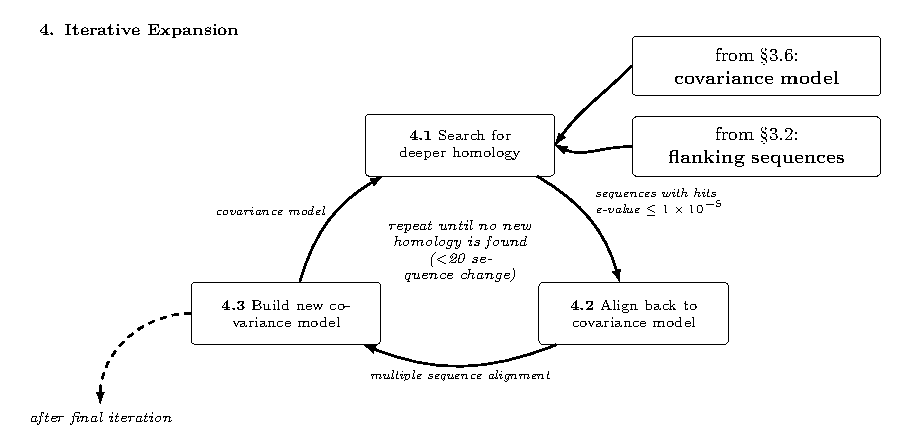
\includegraphics[width=0.95\textwidth]{figures/methods/section4_iterative_expansion.pdf}
    \caption[Iterative expansion of candidate covariance models]{%
    \textbf{Iterative expansion of candidate covariance models.}
    Each covariance model from \S\ref{sec:build_cm} is used to search the flanking sequences from \S\ref{sec:flanking} for deeper homology (4.1) with Infernal v1.1.5. 
    Sequences with hits at an $E$-value $\leq 1\times10^{-5}$ are aligned back to the covariance model (4.2), and a new covariance model is built from the resulting multiple sequence alignment (4.3). 
    The cycle repeats until $<$20 new homologous sequences are found. 
    The dashed arrow marks exit from the loop after the final iteration.}
    \label{fig:iterative-expansion}
\end{figure}

For all uses of this iterative expansion pipeline, a convergence cut-off of 20 new sequences identified in a round was used.
This was to avoid long or infinite iterations.
When this convergence limit was met a final covariance model and alignment was returned as output.

\subsection{Search for deeper homology}

The probabilistic models (covariance models) built by the discovery pipeline were used to search for further homologous sequences in the flanking sequence set (Infernal v.1.1.5 \emph{cmsearch}).
An $E$-value threshold of $1\times 10^{-5}$ was applied to retain significant hits, with otherwise default parameters.
Resulting identified sequences were aligned back to the covariance model.

\subsection{Align back to covariance model}

Infernal v.1.1.5 \emph{cmalign} was used to align identified homologous sequences back to the covariance model of interest \citep{Nawrocki2013}.
This produces a structure-annotated \ac{MSA} of the identified sequences, which can be used to build a new covariance model, potentally adding new structural and sequence information.
These alignments were generated with default parameters as structure-annotated, Stockholm-formatted \acp{MSA}.

\subsection{Build new covariance model}

Probabilistic models describing the structure and sequence of the RNA homology identified in the previous steps were built.
Infernal v.1.1.5 \emph{cmbuild} and \emph{cmcalibrate} were used to build and calibrate new models from the expanded \acp{MSA} \citep{Nawrocki2013}.
Structure was preserved between rounds with the \emph{cmbuild} \texttt{-{}-hand} option, and default \emph{cmcalibrate} parameters.

\subsection{Analysis}

The iterative expansion pipeline outputs are structure-annotated, Stockholm-formatted \acp{MSA}s and calibrated covariance models.
Reported also are the number of rounds of expansion, and the number of sequences identified in each round.
Analysis of the output covariance models was done with the covariance model clustering pipeline (Section~\ref{sec:cm-simile}).
\ac{MSA}s resulting from positive control candidates of the discovery pipeline were also analysed for hit identity and coverage.
Hit identity was calculated as the number of identical sequences between alignments.
Coverage identity was calculated using the coordinates of the alignment sequences, as the number of identical nucleotides between alignments divided by the total length of all alignment sequences.
This was calculated as the intersection / union of the alignment coordinates.
All analysis was done with custom R v.4.6.1 scripts, and plotted with ggplot2, available in the supplementary materials (Appendix~\ref{sec:code-and-data-availability}) \citep{Wickham2016}.

% -------- cm-simile ------------

\section{Covariance model clustering}

An overview of the approaches taken to quantify relatedness between covariance models is provided in Figure~\ref{fig:cm-similarity-approaches}.
These approaches were developed to quantify relatedness between covariance models, and to cluster them based on this relatedness.
This is described in more detail in the following subsections.

\begin{figure}[htbp]
    \centering
    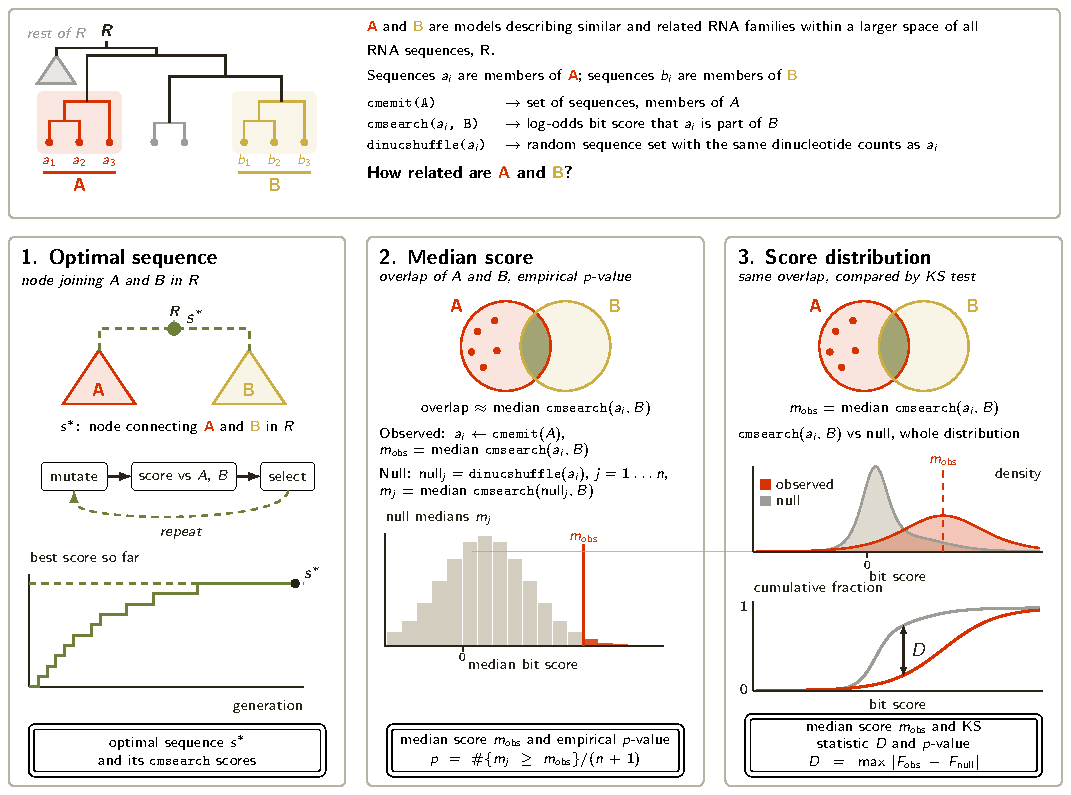
\includegraphics[width=1\textwidth]{figures/methods/section5_cmsimile_approaches.pdf}
    \caption[Approaches for quantifying relatedness between covariance models]{%
    \textbf{Three approaches for quantifying how related two covariance models are.}
    Models $A$ and $B$ describe related RNA families within the space of all RNA sequences, $R$; sequences $a_i$ are members of $A$ and $b_i$ are members of $B$. 
    Sequences are sampled from a model with \emph{cmemit}, scored against a model with \emph{cmsearch} (log-odds bit score), and null sequences are generated by dinucleotide shuffling.
    \textbf{(1) Optimal sequence:} an evolutionary search mutates candidate sequences, scores them against both $A$ and $B$, and selects the best, repeating over generations to approximate the sequence $s^{*}$ that joins the two families; the scores of $s^{*}$ against each model are reported.
    \textbf{(2) Median score:} the median bit score of sequences emitted from $A$ and searched against $B$ ($m_{obs}$) is compared with the medians of $n$ bootstrap resamples of the pooled scores of dinucleotide-shuffled sequences ($m_j$), giving an empirical $p$-value, $p = (1 + \#\{m_j \geq m_{obs}\})/(n + 1)$.
    \textbf{(3) Score distribution:} the full distribution of bit scores is compared with the null using a two-sample Kolmogorov--Smirnov test, where the statistic $D$ is the maximum difference between the observed and null cumulative distributions.}
    \label{fig:cm-similarity-approaches}
\end{figure}

\subsection{Sequence scoring}
\label{sec:sequence-scoring}

Sequences were scored against each model with the Infernal v.1.1.5 tool \emph{cmsearch}, giving a log-odds bit score for each sequence against each model.

\begin{equation} 
S_{\mathrm{bit}}(x)
=
\log_2
\left[
\frac{P(x \mid A)}
     {P(x \mid \varnothing)}
\right]
\end{equation}

where $x$ is a sequence, $A$ is a covariance model, and $\varnothing$ is the null model of random sequence.

\subsection{Sequence sampling}
\label{sec:sequence-sampling}

Sequences were sampled from each probabilistic model (covariance model) with the Infernal v.1.1.5 tool \emph{cmemit}.

\subsection{Null sequence pool generation}
\label{sec:dinuc-shuffle}

Null sequences were generated by an implementation of the Dinucleotide Shuffle algorithm first described by \citet{Altschul1985}.
This approach preserves 2-mer composition while destroying any underlying structure or sequence conservation.

\subsection{Pairwise similarity scoring approaches}

\subsubsection{Optimal sequence}
\label{subsubsec:optimal-sequence}

This approach approximates a shared ancestor, finding a single sequence that can score highly with both models at once, based on the comparison approach by \citet{Eggenhofer2013}.
The optimal sequence, $s^{*}$, was approximated for each pair of models with an evolutionary algorithm.
The initial population was seeded with the consensus sequence of each model and 15 sequences sampled from each model (Section~\ref{sec:sequence-sampling}) [, and filled to a population size of 40 by \ldots].
In each of 15 generations, every sequence was scored against both models (Section~\ref{sec:sequence-scoring}), and the top 25\% by the lower of the two bit scores were retained as survivors and parents.
The population was then restored to its original size with children, each produced either by crossover of two survivors (probability 0.3) or by mutating one survivor (probability 0.7).
Mutation was by point substitution: two positions chosen uniformly at random were each replaced with a nucleotide drawn at random, so sequence length was not changed by mutation.
The search ran for a fixed number of generations, and the highest-scoring sequence found was taken as $s^{*}$.
As the search is stochastic and limited in depth, $s^{*}$ approximates the optimum and its scores are a lower bound on those of the true optimal sequence.

To make scores comparable between pairs of models, the summed bit score of $s^{*}$ against both models was normalised by the scores each model gives its own sequences, to give a similarity ratio,
\begin{equation}
  \label{eq:similarity-ratio}
  \mathrm{SR}(A, B) = \frac{s(s^{*}, A) + s(s^{*}, B)}{\bar{s}_{A} + \bar{s}_{B}}
\end{equation}
where $x_1,\dots,x_N$ are sequences emitted from model $X$, so that $\bar{s}_{X}$ is the mean self score of $X$.
A ratio near 1 indicates that a single sequence scores about as well against both models as typical members score against their own.
Implementation with a custom Go v.1.27.1 code.

\subsubsection{Median score and empirical p-value}
\label{subsubsec:median-score}

This approach asks how well do the sequences of one family fit into another, and vice versa.
300 sequences were sampled from each family (Section~\ref{sec:sequence-sampling}) and scored against the other model (Section~\ref{sec:sequence-scoring}).

% Notation
Let $a_1,\dots,a_N$ be sequences emitted from model $A$, and let $s(x, B)$ denote the \emph{cmsearch} log-odds bit score of sequence $x$ against model $B$.

% Observed statistic
\begin{equation}
  \label{eq:m-obs}
  m_{\mathrm{obs}} = \mathrm{median}_{i=1,\dots,N}\; s(a_i, B)
\end{equation}

To generate a null sequences the sampled sequences were dinucleotide shuffled (\ref{sec:dinuc-shuffle}).
Null populations were bootstrapped from this pool with replacement and median bit scores were used to generate an empirical p-value (all with custom implementations in Go v.1.27.1).

% Null pool
Each $a_i$ is dinucleotide-shuffled once, $\tilde{a}_i = \mathrm{dinucshuffle}(a_i)$, giving a null pool of the same size as the observed set,
\begin{equation}
  \label{eq:null-pool}
  \mathcal{P} = \left\{\, s(\tilde{a}_i, B) : i = 1,\dots,N \,\right\}.
\end{equation}

% Bootstrap null medians
For $j = 1,\dots,n_{\mathrm{boot}}$, a bootstrap population $\mathcal{P}^{*}_j = \{x^{*}_{j,1},\dots,x^{*}_{j,N}\}$ is formed by drawing $N$ scores from $\mathcal{P}$ uniformly with replacement, with median
\begin{equation}
  \label{eq:boot-median}
  m_j = \mathrm{median}\!\left(\mathcal{P}^{*}_j\right), \qquad j = 1,\dots,n_{\mathrm{boot}}.
\end{equation}

% Empirical p-value
\begin{equation}
  \label{eq:empirical-p}
  p = \frac{1 + \#\{\, j : m_j \geq m_{\mathrm{obs}} \,\}}{n_{\mathrm{boot}} + 1}
\end{equation}

The reported metric of this approach is the sum of $m_{\mathrm{obs}}$ for both directions to give a single pair value.

\subsubsection{Score distribution}
\label{subsubsec:score-distribution}

The third approach taken was driven by an observation that although the magnitude of $m_{\mathrm{obs}}$ (Equation~\ref{eq:m-obs}) is often small between same clan RNA families (Section~\ref{subsec:clan-benchmark}), distributional differences between $s(a_i, B)$ and $s(\tilde{a}_i, B)$ can still be seen. 
The two-sample \ac{KS} test \citet{Smirnov1939} was applied to the observed scores $s(a_i, B)$ and the null pool $\mathcal{P}$ (Equation~\ref{eq:null-pool}), both of size $N$. 
The test statistic, $D$, is the maximum vertical distance between the empirical cumulative distribution functions of the two sets. 
It was computed using a custom Go v.1.27.1 implementation and is denoted $D_{A into B}$ for sequences emitted from $A$ and scored against $B$.
Reported combined score is simply $D_{A into B} + D_{B into A}$, used in the preliminary clan benchmark.

\subsection{Analysis}
\label{subsec:clustering-analysis}

To test the practicality and performance of the pairwise similarity scoring approaches, two complementary tests were performed: one assessed whether curated relatedness could be recovered, and the other whether fragments of a fractured RNA family could be identified as such.
All curation and annotation sets and results are available (Appendix~\ref{sec:code-and-data-availability}).

Data handling and plotting were done in R v.4.6.1 using the readr and ggplot2 v.4.0.3 packages \citep{Wickham2016}.
Clustering was computed by pairwise distance and plotted with a dendrogram.
Plotting and summary functions are available in the repository (Appendix~\ref{sec:code-and-data-availability}).

\subsubsection{Clan benchmark}
\label{subsec:clan-benchmark}

Rfam families are curated into clans where they are deemed to be related and share common ancestry \citep{Ontiveros-Palacios2025}.
A set of 44 families from various clans was curated from Rfam (version 15.0) to test whether the pairwise similarity approaches could recover clan relationships.
All 946 possible pairs of families were scored with each approach.

Separation of within-clan from other pairs was quantified as the area under the receiver operating characteristic curve (AUC), calculated from ranks as \
$\mathrm{AUC} = U / (n_{\mathrm{within}}\, n_{\mathrm{other}})$, where $U$ is the number of (within-clan, other) pairs of pairs for which the within-clan pair has the higher statistic, counting ties as one half. 
This is the probability that a randomly chosen within-clan pair outscores a randomly chosen other pair. 
An AUC of 0.5 indicates no separation and 1 indicates perfect separation. 
The AUC makes no assumption about the distribution of the statistics and is unaffected by their scale. As pairs sharing a family are not independent, 95\% confidence intervals were obtained by bootstrapping over families.


\subsubsection{PROBABLY WILL REMOVE AS I DONT TALK ABOUT Fractured model}
\label{subsec:fractured-fmn-test}

The use case of this clustering in this study was to identify candidates yielded by the discovery pipeline that describe the same signal.
As such it made sense to test if the pairwise similarity scores identified similarities in covariance models describing the same underlying signal.
The Rfam annotated \ac{FMN} seed sequences (Section~\ref{subsec:covariance-models}) were clustered, aligned, structure predicted and built into covariance models as in the final steps of the computational discovery pipeline (Sections~\ref{subsec:clustering}, \ref{subsec:rna-alignment}, \ref{subsec:covariance-analysis} and \ref{sec:build_cm}).
This set of \acp{CM} provided a test set for similarity scoring.

% \subsubsection{Score distribution}
% \label{subsubsec:score-distribution}

% The third approach taken was driven by an observation that although the magnitude of $m_{\mathrm{obs}}$ (Equation~\ref{eq:m-obs}) is often small between same clan RNA families (\ref{subsec:covariance-models}), distributional differences between $s(a_i, B)$ and $s(\tilde{a}_i, B)$ can still be seen.

% % KS statistic
% Let $F_{\mathrm{obs}}$ and $F_{\mathrm{null}}$ be the empirical cumulative distribution
% functions of the observed and null scores, with indicator function $\mathbf{1}[\cdot]$,
% \begin{equation}
%   \label{eq:F-obs}
%   F_{\mathrm{obs}}(x) = \frac{1}{N} \sum_{i=1}^{N} \ind{s(a_i, B) \leq x}
% \end{equation}
% \begin{equation}
%   \label{eq:F-null}
%   F_{\mathrm{null}}(x) = \frac{1}{N} \sum_{y \in \mathcal{P}} \ind{y \leq x}
% \end{equation}
% and the Kolmogorov--Smirnov statistic is
% \begin{equation}
%   \label{eq:ksd}
%   D = \max_{x} \left| F_{\mathrm{obs}}(x) - F_{\mathrm{null}}(x) \right|.
% \end{equation}


% The two-sample \ac{KS} statistic, $D$ (Equation~\ref{eq:ksd}), was used to quantify the difference between the distribution of bit scores obtained by searching sequences emitted from model $B$ against model $A$ and the distribution obtained from their dinucleotide-shuffled counterparts. 
% This value is denoted $D_{B into A}$.

% -------- ethics n stuff ------------

\section{Ethics, MPI and EPA regulations}

This project uses publicly available genomic sequence data and does not involve human participants, animal experimentation, or the construction of genetically modified organisms.

No ethical approval, MPI, or EPA approvals are required at this stage. 
Should the scope expand to require these approvals, they will be sought.
